\chapter{\label{detchar}Detector Characterisation with SOAP}
%%%%%%%%%%%%

When searching for \ac{GW} signals, it is important to understand the origins of noise in the the detectors data which does not originate from an astrophysical source.
A large fraction of \ac{GW} search algorithms, including SOAP above, assume that the detectors noise follows a Gaussian distribution.
However, the detectors contain artefacts which are not distributed as a Gaussian. 
These artefacts can negatively affect many searches for \ac{GW} as they can be easily mistaken for a real \ac{GW} signal.
Some of the potential sources of these artefacts have been mentioned in Sec.~\ref{intro:detector:noise}. 
There are many different classes of artefact, some key types include: glitches, these are short duration signals and instrumental lines which are long duration.
To conduct a reliable search there are two main tasks which are necessary for detector characterisation.
The first is identifying the artefact such that any search knows that part of data is contaminated.
The search can then remove that section of data, or use more sophisticated techniques to deal with the artefact \citep{}.
The second task is to find the source of the artefact. 
If the source of the artefact is found, it can potentially be removed or limited for future data runs.

The focus of this chapter is on a particular class of artefact called instrumental lines and how the affect \ac{CW} searches.
Sec.~\ref{detchar:lines} will introduce different classes of instrumental line and how it affects a \ac{CW} search.
Sec.~\ref{detchar:monitor} will outline how these artefacts are detected and monitored, and describe current tools used for this task.
Sec.~\ref{detchar:soap} will describe how the \ac{CW} search algorithm introduces in Sec.~\ref{soap} can be used to search for instrumental lines.
Finally Sec.~\ref{detchar:summary} will show the outputs of the search and this is displayed for ease of use.



%%%%%%%%%
%%%%%%%%%%
\section{\label{detchar:lines}Instrumental lines}
%%%%%%%%%
%%%%%%%%%

Instrumental lines have the general structure that they are persistent noise artefacts.
There are many classes of instrumental line including: narrow, fixed frequency spectral artefacts or broad features which have a time varying frequency known as wandering lines.
Many of these lines can make it difficult to distinguish them from an astrophysical signal.
For many search methods, lines affect results in two main ways. 
They can cause the search to produce outliers which are considered as \ac{GW} candidates.
If the line is close to the \ac{GW} signal in frequency, then it can conceal the power of the \ac{GW}, or if it is overlapping, the search can be almost impossible.
It is therefore crucial to understand the structure and origin of these lines when performing a search for \ac{GW} specifically \ac{CW} and stochastic searches.

Some instrumental lines are clearly visible when looking at one fo the \ac{LIGO} detectors frequency spectrum is shown in Fig.~\ref{detchar:line:psd}. This figure demonstrates some lines which have larger amplitudes. There are however, many more weaker line which become visible when spectra are averaged over longer times.
\begin{figure}
    \centering
    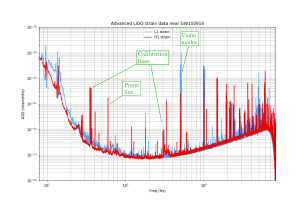
\includegraphics[width=\textwidth]{C5_detchar/ligo_o1_asd_annot.pdf}
    \caption{There are many features in the \ac{LIGO} detectors averaged spectral density. This image was taken from \citep{GWOpen} where I have annotated some of the stronger lines. The power line from the mains in the USA is at 60 Hz. Some of the calibration lines are around 30 Hz, 331 Hz and 1083 Hz. The various violin modes of the suspensions are at 300, 500, 600 and 900 Hz where I have only marked the 500 Hz mirror suspension modes \citep{GWOpen}.}
    \label{detchar:line:psd}
\end{figure}
The frequency spectrum in Fig.~\ref{detchar:line:psd} shows the time averaged spectra the \ac{GW} channel of the \ac{LIGO} detectors. 
The lines seen in the spectrum are not from any \ac{GW} and are usually from ground based sources.
To see the lines in the \ac{GW} channel, they must be coupled in via some mechanism. 
There are a number of ways in which this happens which are outlined in \citep{covas2018IdentificationMitigation}.
This includes coupling via shared power and grounds. 
When different components share the same power supplies, if a component draws power with a given period, then the voltage will decrease at this frequency. 
Another component which shares this same power supply can then also see this drop in voltage and this can potentially affect a stored output. 
Another mechanism is coupling through magnetic fields, this is common when cables are nearby and can couple the magnetic field to different systems.
Coupling can also occur though a physical connection, known as mechanical coupling, for example the resonances of the suspension fibres which couple directly to the mirrors.

Many of the spectral lines seen in the frequency spectrum, Fig.~\ref{detchar:line:psd} are fundamental to the design of the detector. 
These cannot be eliminated, therefore need to be understood such that their effect on searches in minimised.
Some of these lines are listed below.
\begin{description}
	\item[Power line] The power line harmonics are fundamental to the detector and originate from the US mains supply. These lines exist at 60 Hz which is the frequency of the mains alternating current oscillates at \citep{aasi2015CharacterizationLIGO}.
	
	\item[Violin modes] The violin modes are associated with the suspensions of the mirrors and the beam splitter in the detector. These are designed to have a narrow frequency spectrum such that they contaminate as smaller part of the spectrum as possible. These are the lines around 500 Hz for the mirrors and 300, 600 and 900 Hz for the beam-splitter \citep{GWOpen} in Fig.~\ref{detchar:line:psd}.
	
	\item[Calibration lines] The mirrors of the \ac{LIGO} detectors, are held at a resonance of the cavity in the arms of the interferometer. This then requires a feedback loop to hold them at resonance as a \ac{GW} passes the detector. Calibration lines are used to calibrate this feedback loop such that the arm length changes are accurate \citep{tuyenbayev2016ImprovingLIGO,coughlin2010NoiseLine}.
\end{description}
In \citep{davis2019ImprovingSensitivity}, techniques to counter the affect of power lines and calibration lines. 

Along with the fundamental lines of the detector which cannot be removed at the source, there are a large number of other lines whose source has been found and can be removed. 
Many of these are from mechanisms described earlier such as shared power supplies or grounds, these can be removed by, for example, using a different supply for different systems.

These lines have large effect on all searches for \acp{GW} both if the astrophysical signals frequencies overlap with the frequency of the line and can cause outliers. 
Long duration searches for \acp{CW} are particularity sensitive to this type of artefact.
As described in Sec.~\ref{searchcw}, \ac{CW} are long duration signals with a slowly varying frequency.
In the case of an isolated neutron star, the signal which is searched for is narrow-band and a fixed frequency which is Doppler modulated by the earths rotation and orbit.
For certain areas of parameter space, the astrophysical signal of an isolated neutron star can appear very similar to an instrumental line. 
Many of these lines can be mitigated by using multiple detectors data. If a signal appears in a one detector and not the others, then it is likely that the signal is from an instrumental lines. 
These contaminated frequency bands can be removed of a statistic similar to that described in Sec.~\ref{viterbi:las} or \citep{keitel2014SearchContinuous} can be used to limit their effect.
However, there are many examples of instrumental line which appear at the same or similar frequencies in multiple detectors.
These pose a real challenge to some \ac{CW} searches, and require a lot of investigation to limit their affect.

%%%%%%%%%%
%%%%%%%%%%
\section{\label{detchar:monitor}Identifying and monitoring instrumental lines}
%%%%%%%%%%
%%%%%%%%%%

When a detector is running, it is very important to identify instrumental lines and monitor them.
This can then lead to either locating the origin of the line such that it can be removed, or allowing it to be flagged for other search algorithms.
The lines are generally identified in the \ac{GW} channel, this is the output of the detector which \ac{GW} are observed and is the data using is previous chapters.
This is the channel where the affect of lines is intended to be minimised.

As well and the \ac{GW} channel the detector records many different channels known as auxiliary channels. 
These channels monitor many components of the detector.
For example, the seismometers which are located near the corner stations and end stations are all channels which are monitored. 
There are magnetometers located around the electronics on the site to measure how these may be affecting the detector. 
These channels can be very useful in identifying the source of an instrumental line.
These channels which monitor the environment are known as \ac{PEM}.
The main goal is to reduce the number of artefacts in the \ac{GW} such that it is as close to Gaussian noise as possible.
If an artefact shows up in the \ac{GW} channel in coincidence with one of the \ac{PEM} or other channels, then this is an indicator that the artefact originates from something related to that \ac{PEM}.
For example, say a magnetometer located near some electronics has a long duration line in its spectrum at the same frequency as the main \ac{GW} channel. 
This indicates that the magnetic field of that piece of electronics is somehow coupling into the detector. 

There are a number of tools which are used to monitor these spectral lines, along with a team of people which regularly look though the results, a summary of these for the first two observing runs of \ac{LIGO} can be found in \citep{covas2018IdentificationMitigation}.
Some of the tools used are described below. 

\begin{description}
	\item[Fscan] Fscan \citep{coughlin2010NoiseLine} takes \acp{FFT} of the raw detector data, typically these are 1800s long. This is done for all of the auxiliary channels as well as the \ac{GW} channel. The \acp{FFT} are then averaged over a day and spectrograms are generated. After known lines such as Violin modes and power lines are subtracted, noise lines can be identified. A threshold can be set and anything in the spectrograms which exceed this threshold are flagged as a line. These can then be compared across multiple different channels. More detail on how the lines are identified can be found in \citep{coughlin2010NoiseLine}
	
	\item[Coherence] Coherence searches for the coherence between different channels and different detectors. This is similar to searches for stochastic gravitational waves. More detail of how this works can be found in \citep{covas2018IdentificationMitigation}
	
	\item[Finetooth] Many of the instrumental lines found are part of combs. These are repeating structures where the harmonics (teeth) of a line make up the comb which is defined by the start frequency and tooth spacing. Finetooth is a tool which identifies and monitors these combs \citep{}.
	
	\item[NoEMi] NoEMi uses \acp{FFT} and identifies peaks within the spectrum. I can then find coincidences with auxiliary channels and label is there are overlapping peaks with the \ac{GW} channel. This can then tracks the lines with time. All of the information is stored in a database where more detail on its operation can be found in \citep{accadia2012NoEMiNoise}.
	
\end{description}

These tools offer many ways for the detector characterisation team to identify instrumental lines and hunt for their source. A summary of these efforts for the advanced \ac{LIGO} data can be found in \citep{covas2018IdentificationMitigation}.
The following sections describe how the SOAP search described in Sec.~\ref{soap} can be used as an extra tool to aid in the identification and monitoring of instrumental lines.

%%%%%%%%%%%
%%%%%%%%%%%
\section{\label{detchar:soap}Identifying and cleaning lines with SOAP}
%%%%%%%%%%%
%%%%%%%%%%%%

The SOAP search has been run on a number of observing runs to search for \ac{CW}. 
One of the major factors which limited the sensitivity of the search is instrumental lines. 
Whilst for the majority of this thesis I have worked on developing techniques to limit the affect instrumental lines, the search also has the ability to identify these lines well.
In this section, I will explain the setup of the search to identify instrumental lines.

Sec.~\ref{soap} described how multiple detectors can be used to increase the sensitivity of a search for \acp{CW}. 
However, when searching for instrumental lines, the aim is to have the reverse effect, therefore, a simple search is run separately on each detector. 
This then removed any of the statistics developed in Sec.~\ref{viterbi:las} and uses the \ac{FFT} power as the statistic in the SOAP search.
The single detector soap search then has one parameter to vary, the transition matrix parameter. 
This governs how probable the frequency track is to transition up straight or down a frequency bin.
In this search we are aiming to find any non Gaussian artefacts, therefore, we allow an equal probability for the track to jump in any direction. 
The Fscan search described above generates \acp{FFT} every day of varying lengths, this include 1800 s long \acp{FFT}. 
We use this to our advantage as the search is already set up to search through 1800 s long time-frequency spectrograms. 
For this line search, we split the 1800 s long Fscan \acp{FFT} into 0.2 Hz wide sub-bands and run the single detector search on each sub-band. 
This then returns the same outputs as described in Sec.~\ref{soap} and Sec.~\ref{cnn}: the frequency track (Viterbi track), a Viterbi map and a Viterbi statistic. 
Here the Viterbi statistic is just the sum of the \ac{FFT} power along the frequency track. 
This outputs a plot as shown in Fig.~\ref{detchar:soap:exampleplot}.
\begin{figure}
	\centering
	\includegraphics[width=\textwidth]{testimg.png}
	\caption{Example of output plot from SOAP line search.}
	\label{detchar:soap:exampleplot}
\end{figure}

The Viterbi statistics are then ranked in order, where the largest value is most likely to be from and instrumental artefact. 
The top results can be compared to the known line lists from the other line tools mentioned in Sec.~\ref{detchar:monitor}.



\begin{figure}
	\centering
	\includegraphics[width=\textwidth]{testimg.png}
	\caption{different types of instrumental line which appear in SOAP spectrograms}
	\label{detchar:line:psd}
\end{figure}

\begin{itemize}
    \item overview of soap search and what type is used for line searches
    \item how this is applied and how to interpret the output for lines searches
    \item SOAP can identify weak lines when they are wandering or fixed frequency
    \item 
\end{itemize}


%%%%%%%%%%%
%%%%%%%%%%%%
\section{\label{detchar:summary}Summary pages}
%%%%%%%%%%%
%%%%%%%%%%%%%

Summary pages are an important tool when searching for instrumental lines. 
There is such a large amount of data both in frequency and time space and channels to search though when looking for instrumental lines.
Summary pages should provide an easy way to view the important information to identifying the line as well as be easy to navigate to find a particular area of the spectrum which is of interest. 
These summary pages exist for the above searches in \citep{line summary pages}.

For the SOAP search summary pages were generated for each observing run and for the two \ac{LIGO} detectors. 
This was done for various timescales: for the entire observing run and separately for each month.
This allows the variation of a line to be observed for the entire length and also artefacts on shorter timescales to be observed.
An example of the output plot is shown in Fig.~\ref{detchar:summary:plots} for the entire O1 observing run.
The plots three main panels which are explained below.
\begin{description}
	\item[Spectrograms] The time-frequency spectrograms show the power spectrum of the 1800 s \acp{FFT}. The optimal Viterbi track is then overlaid on top.
	
	\item[Viterbi maps] The Viterbi maps show the `log-probability' of a signal being present in any particular frequency bin at a given time. This can be thought of as a distilled view of the spectrograms above.
	
	\item[Sensitivity and power] The final panel in the example plots show an estimate of the sensitivity with time. The plot also shows the \ac{FFT} power along the optimal tracks path. This allows the user to see how the sensitivity varies with the spectrogram power along the signal track. This can be useful when trying to identify some spectral artefacts.
\end{description}

\begin{figure}
	\centering
	\includegraphics[width=\textwidth]{testimg.png}
	\caption{example plot of the summary pages}
	\label{detchar:summary:plots}
\end{figure}
\begin{itemize}
    \item why summary pages are useful 
    \item how to read them and what they mean
    \item how to use the information with other searches
\end{itemize}
